\chapter{Resource Description Framework}

Semantic web uses URI to identify an existing interpretation, RDF/RDFS to store semantics, OWL to enforce complex logic, and SPARQL to query and manipulate the database. 

RDF, RDFS and basic SPARQL are introduced in this chapter. OWL will be introduced in the next Chapter \ref{ch:owl}.

\section{Uniform Resource Identifier} \label{sec:uri}

Human uses symbols to represent objects in reality. The concept associated with a symbol is used to help define and interpret objects. An example of interpreting ``Apple'' is given in Fig. \ref{fig:semiotictriangle}.
\begin{figure}[!htb]
	\centering
	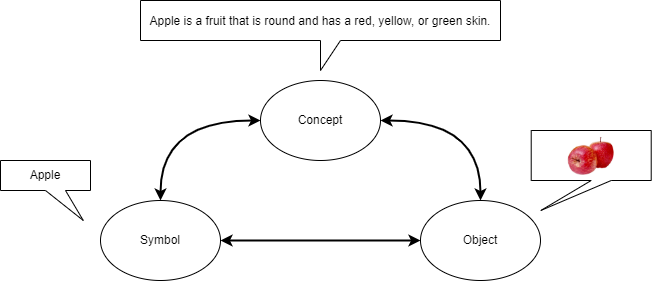
\includegraphics[width=0.8\textwidth]{chapters/part-4/figures/semiotic_triangle.png}
	\caption{Semiotic triangle of Apple.}
	\label{fig:semiotictriangle}
\end{figure}

\mync{Uniform resource identifier}[URI] points to the interpretation of the symbols used in the semantic web. In practice, the resource is either the definition of the class/object/property, or the higher-level ontology (often by another semantic web). For example, consider building a semantic web to describe an apple farm. Consider using \texttt{dbpedia.org/page/Apple} from DBpedia as the URI of interpretation of apple, which already gives a clear and rich definition of apple such as abstract, Wikipedia link, emoji, sugar level, etc. This saves the time of building the interpretation of apple from scratch. 

URI can be used to bridge multiple semantic webs and build semantic web hierarchy, by doing which the system is naturally merged and scaled up.

URI shall contain at least two pieces of information: the address (locator), and the identity (name). URI is often ASCII encoded, but it is possible to extend to unicode. The generic syntax is given below. If it looks similar with the \myabb{Uniform Resource Locator}{URL}, that is because URL is considered as a subclass of URI.
\begin{lstlisting}
scheme:[//authority]path[?query][#fragment]
\end{lstlisting}
where
\begin{itemize}
\item \verb|scheme| specifies the protocol used to access the resource. Common schemes include \verb|http|, \verb|https|, \verb|ftp|, \verb|mailto|, \verb|file|, and \verb|data|. The scheme is followed by a colon \verb|:|.
\item \verb|authority| specifies the user information, host, and port, separated by \verb|@| and \verb|:|, respectively. The authority is preceded by a double forward slash \verb|//|.
\item \verb|path| identifies the specific resource within the context of the scheme and authority. It is a sequence of segments separated by forward slashes \verb|/|.
\item \verb|query| provides additional information that the resource can use for processing. It is a series of key-value pairs separated by an ampersand \verb|&|. The query starts with a question mark \verb|?|.
\item \verb|fragment| identifies a specific part or section within the resource. It is typically used with HTML documents to indicate a specific anchor or location within the page. The fragment starts with a hash sign \verb|#|.
\end{itemize}
More details can be found at
\begin{lstlisting}
https://www.rfc-editor.org/rfc/rfc3986.html#section-3.1
\end{lstlisting}
which happens to be a good example of an URI.

\section{Resource Description Framework} \label{sec:rdf}

RDF is the backbone data model of the semantic web. It stores data in the form of triples. RDF alone is not powerful enough to record \myabb{description logic}{DL}. In practice, RDF usually works with RDFS which expands its vocabulary to include class, subclass, etc., and OWL which further expands its vocabulary and introduce \myabb{description logic}{DL} features, to together form a comprehensive semantic web. RDF is the fundamental of RDFS and OWL.

Notice that RDF is not a syntax by itself. A markup language is needed to host the RDF framework. Commonly used markup languages are listed below. They can be translated from one to the other.
\begin{itemize}
  \item RDF/XML: has good compatibility with old machines.
  \item \myabb{Terse RDF Triple Language}{Turtle}: easy to use, human-readable.
  \item \myabb{JSON for Linked Data}{JSON-LD}: popular in web applications and APIs where JSON-based format is required.
  \item N-Triples: simple, machine-readable format for data exchange between tools.
\end{itemize}
Unless otherwise mentioned, Turtle is used in this notebook.

\subsection{Triple Representation}

RDF uses ``subject-predicate(property)-object'' triple to represent knowledge. A triple is corresponding with an edge in a directed graph, which is often used to visualize RDF. 

For example, consider ``Einstein was born in Ulm''. In RDF, ``Einstein'' is the subject, and ``Ulm'' the object. The predicate is ``has birthPlace'', where ``birthPlace'' is a property assigned to ``Einstein''. The graph representation is given by Fig. \ref{fig:einsteinexp}.
\begin{figure}[htbp]
	\centering
	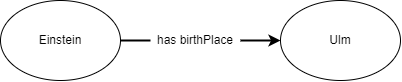
\includegraphics[width=0.6\textwidth]{chapters/part-4/figures/einsteinexp.png}
	\caption{Graph representation of triple for knowledge ``Einstein was born in Ulm''.}
	\label{fig:einsteinexp}
\end{figure}
The RDF in Turtle is given as follows.
\begin{lstlisting}
@prefix dbo: <http://dbpedia.org/ontology/> .
@prefix dbr: <http://dbpedia.org/resource/> .

dbr:Albert_Einstein dbo:birthPlace dbr:Ulm .
\end{lstlisting}
where \verb|Albert_Einstein| and \verb|Ulm| are defined in \verb|dbpedia.org/resource/| as name and place, and \verb|birthPlace| in \verb|dbpedia.org/ontology/| as a property. To breakdown the Turtle in more details:
\begin{itemize}
  \item \verb|@prefix| keyword is used to define prefixes for namespaces, making it easier to write URIs.
  \item \verb|dbr:Albert_Einstein| is the subject, representing Albert Einstein as a resource in the DBpedia namespace.
  \item \verb|dbo:birthPlace| is the predicate, representing the ``birthPlace'' property from the DBpedia ontology.
  \item \verb|dbr:Ulm| is the object, representing the city of Ulm as a resource in the DBpedia namespace.
  \item \verb|.| indicates the end of a statement.
\end{itemize}

Use
\begin{lstlisting}
<subject> <predicate> <object> .
\end{lstlisting}
to claim a statement. When multiple objects are assigned to a subject, consider using
\begin{lstlisting}
<subject> <predicate1> <object1>; <predicate2> <object2>; <predict3> <object3> .
\end{lstlisting}
which is equivalent to
\begin{lstlisting}
<subject> <predicate1> <object1> .
<subject> <predicate2> <object2> .
<subject> <predicate3> <object2> .
\end{lstlisting}

\subsection{Multi-valued Relation and Blank Node}

It is possible to use multi-valued relations and blank nodes to aggregate information. Consider an example given in Fig. \ref{fig:lectureexp}, where the graph is used to demonstrate a lecture taking place at a specific room at given time slot. What if the lecture takes place twice a week, each time at a different location? 

With the help of multi-valued relations and blank nodes, this can be demonstrated clearly as shown in Fig. \ref{fig:lectureexp2}. In this example, blank node plays as an unnamed intermediate node that hosts a nested structure.
\begin{figure}[!htb]
	\centering
	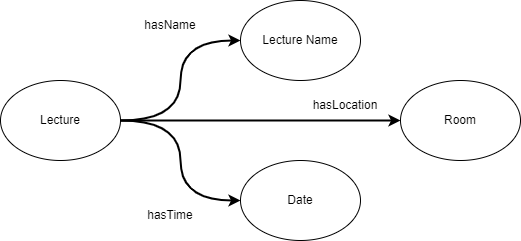
\includegraphics[width=0.6\textwidth]{chapters/part-4/figures/lectureexp.png}
	\caption{An example that demonstrate when and where a lecture takes place.}
	\label{fig:lectureexp}
\end{figure}

\begin{figure}[!htb]
	\centering
	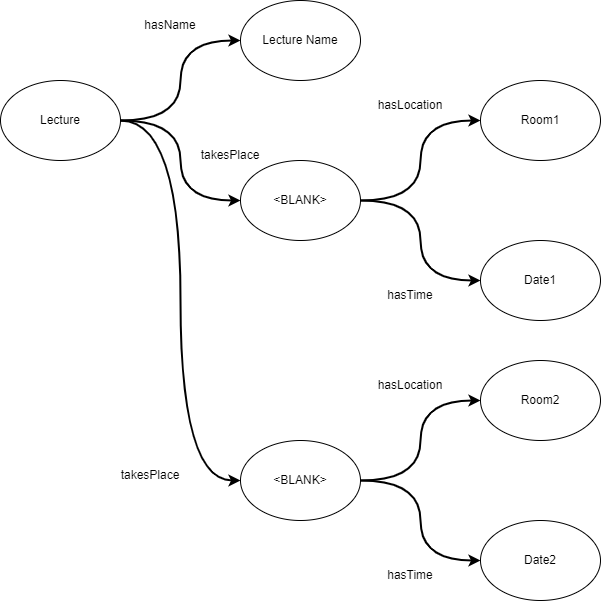
\includegraphics[width=0.6\textwidth]{chapters/part-4/figures/lectureexp2.png}
	\caption{An example that demonstrate a lecture taking place at multiple locations and time slots using multi-valued relations and blank nodes.}
	\label{fig:lectureexp2}
\end{figure}

Turtle and other markup languages provides syntax for creating blank nodes that looks like the following.
\begin{lstlisting}
<subject1> <predicate1> [
	<predicate2> <object2>;
	<predicate3> <object3>
] .
\end{lstlisting}
To refer to a blank node, it is also possible to give the blank node a name. The syntax looks like the following.
\begin{lstlisting}
<subject1> <predicate1> _:<blank-node-name> .
_:<blank-node-name> <predicate2> <object2> .
_:<blank-node-name> <predicate3> <object3> .
\end{lstlisting}
where \verb|_:<blank-node-name>| is used to declare a blank node and assign it a name. For normal nodes URI takes the position of \verb|_|. Bland nodes do not possess a global identifier, and \verb|_:<blank-node-name>| is only a local identifier used in a single RDF script.

\subsection{Lists}

Lists help to make the code clean and readable. There are two types of lists, containers (open list, extendable, unordered or partially ordered) and collections (closed list, well-defined, ordered and fixed). Container is helpful to handle the situation given in Fig.  \ref{fig:lectureexp3}.
\begin{figure}[!htb]
	\centering
	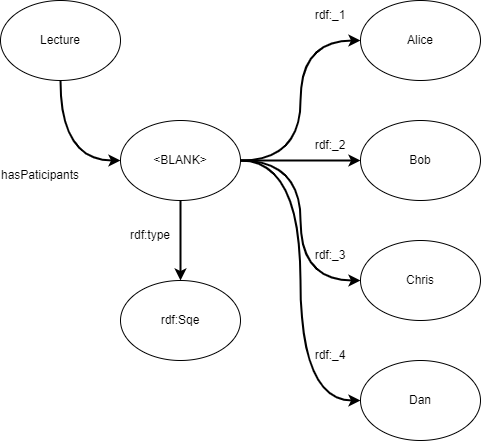
\includegraphics[width=0.6\textwidth]{chapters/part-4/figures/lectureexp3.png}
	\caption{An example of a container.}
	\label{fig:lectureexp3}
\end{figure}
Notice that the blank node has a type \verb|rdf:Seq|. This tells that the items stored in the container follows an ordered set. There are other container types, such as \verb|rdf:Bag| (unordered set) and \verb|rdf:Alt| (alternatives of elements; only one element is relevant for the application).

The collection, on the other hand, defines a closed list as shown by Fig. \ref{fig:lectureexp4}. In Turtle, this can be done by using nested \verb|[]| recursively.
\begin{figure}[!htb]
	\centering
	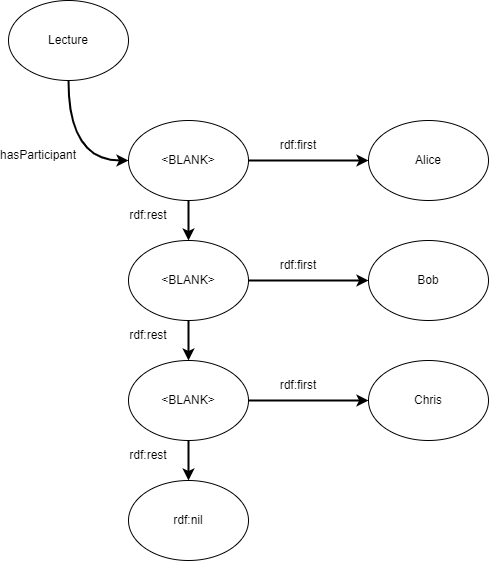
\includegraphics[width=0.6\textwidth]{chapters/part-4/figures/lectureexp4.png}
	\caption{An example of a collection.}
	\label{fig:lectureexp4}
\end{figure}
A short cut is to use \verb|()|, with the items in the collection listed down in the bracket as follows.
\begin{lstlisting}
<subject> <predicate> (<object1> <object2> <object3>) .
\end{lstlisting}

\subsection{Reification}

RDF permits interleaving of statements, i.e., to make a statement about another statement. For example, consider ``Alice says that Bob ate the cake''. This example contains nested statement, where ``Bob ate the cake'' is a statement, and ``Alice says \ldots'' is a statement on that statement. RDF reification follows Fig. \ref{fig:reificationexp}.
\begin{figure}[!htb]
	\centering
	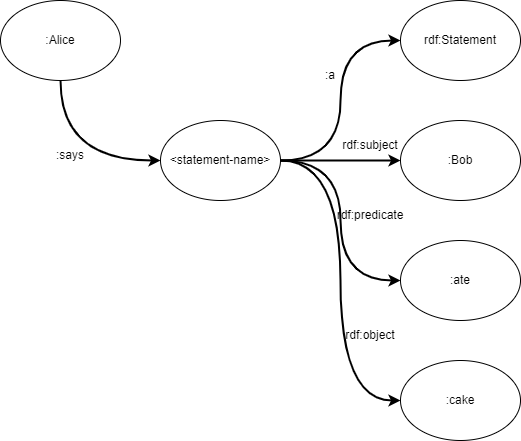
\includegraphics[width=0.6\textwidth]{chapters/part-4/figures/reificationexp.png}
	\caption{An example of RDF reification.}
	\label{fig:reificationexp}
\end{figure}

\subsection{Converting RDB to RDF}

For small-scale relational database, it is possible to convert it to semantic web RDF manually. For example, consider an RDB for all the books in a study. There are three tables in the database, books, authors and publishers, respectively. Each table contains a few dozens of entries. The RDB can be converted to RDF as shown in Fig. \ref{fig:bookexp}. It can be realized very easily, simply by defining everything as nodes and stack triples for all relationships.
\begin{figure}[!htb]
	\centering
	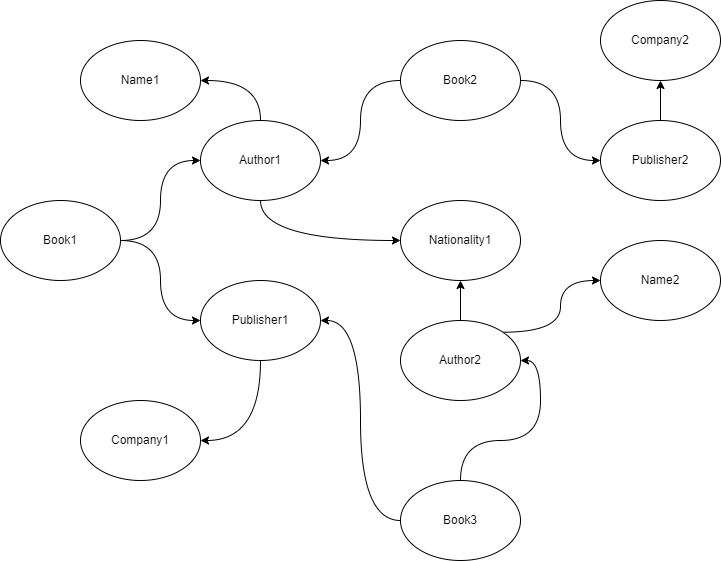
\includegraphics[width=0.8\textwidth]{chapters/part-4/figures/bookexp.png}
	\caption{Semantic web of a few books, and their authors and publishers.}
	\label{fig:bookexp}
\end{figure}

However, when comes to a large and complicated database, converting it to RDF manually would consume too much labor. Several ways to systematically do the conversion have been proposed. Details are not covered here. See \cite{michel2014survey} for more details.

In summary, RDF defines the objects (nodes) and also the properties among objects (edges). This is essentially how RDF differs from a conventional key-value based NoSQL. RDF can be easily scaled up.

The underlying mechanisms behind RDF, such as how machine stores graphical database including nodes and relationships, and how it enables query using SPARQL, is out of the scope of this notebook. Though details are not given, a brief review of the mechanisms is given in later part of the notebook.

\section{RDF Schema} \label{sec:rdfs}

RDFS enforces schema to the RDF model. By using RDF/RDFS, a more consistent and semantic RDF model can be achieved.

\subsection{RDF Versus RDF/RDFS} \label{subsec:rdfvsrdfs}

RDF is flexible. It is so flexible that sometimes it becomes difficult to maintain consistency, let alone performing sophisticated reasoning from it. RDFS enforces schema to the RDF model by adding more ``meta information'' which builds more connections among the nodes.

RDFS expands the vocabulary of RDF. It introduces class and subclass to RDF. It provides built-in predefined classes such as \verb|rdfs:Literal|, \verb|rdfs:Resource|, \verb|rdfs:Datatype|, etc., and enforce the nodes to be linked to these classes. RDF already defines \verb|rdf:Property|. RDFS further expands the properties and relations. All above makes the RDF/RDFS modeling more consistent and semantic than using RDF alone.

In the deeper insights, RDFS helps to add ontology to the RDF model by introducing the schema. It essentially integrate common understanding and domain knowledge to the information. For example, by creating a property ``\verb|:hasSpouse|'' whose domain and range ``person'', it demonstrates the common knowledge that a person can be married to another person.

The following example compares RDF and RDF/RDFS implementations on the same context. Consider statement ``banana is yellow, apple is red, and orange is orange color''. In an RDF implementation, this would look like the green-colored elements in Fig. \ref{fig:fruitexp}. It is a disconnected graph. The semantic web failed to bridge the triples together. Neither is it aware that all of them are discussing colors of fruits.
\begin{figure}[!htb]
	\centering
	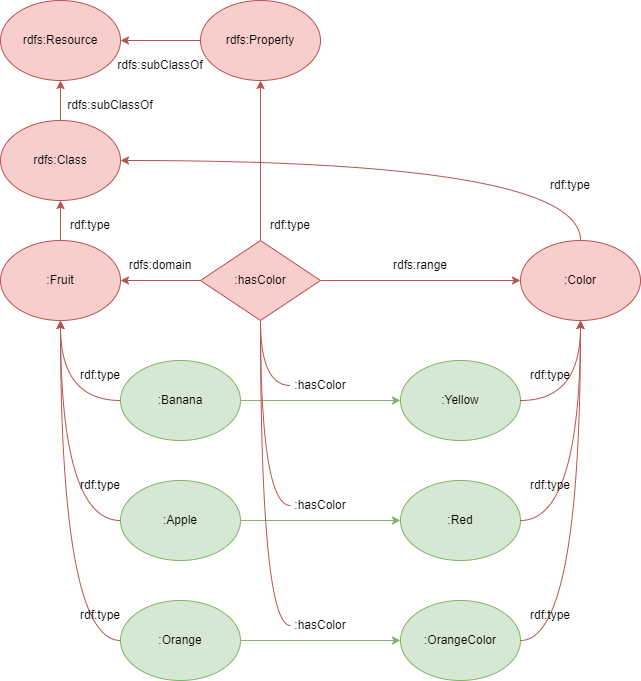
\includegraphics[width=0.8\textwidth]{chapters/part-4/figures/fruitexp.png}
	\caption{Semantic web of fruits and their colors, with RDF implementation in green RDF/RDFS in red.}
	\label{fig:fruitexp}
\end{figure}

In an RDF/RDFS implementation, class/subclass and property are enforced in the RDF model, and each property must be associated with clearly defined domain and range. All classes eventually root to \verb|rdfs:Resource|. This is shown by the green plus red color in Fig. \ref{fig:fruitexp}. The corresponding Turtle is
\begin{lstlisting}
@prefix rdf: <http://www.w3.org/1999/02/22-rdf-syntax-ns#> .
@prefix rdfs: <http://www.w3.org/2000/01/rdf-schema#> .
@prefix example: <http://example.org/> .

# Define classes (optional; they are implicit)
rdfs:Class rdfs:subClassOf rdfs:Resource .
rdf:Property rdfs:subClassOf rdfs:Resource .

example:Fruit rdf:type rdfs:Class ;
rdfs:subClassOf rdfs:Resource .

example:Color rdf:type rdfs:Class ;
rdfs:subClassOf rdfs:Resource .

# Define properties
example:hasColor rdf:type rdf:Property ;
rdfs:domain example:Fruit ;
rdfs:range example:Color .

# Define fruits and colors
example:Banana rdf:type example:Fruit .
example:Apple rdf:type example:Fruit .
example:Orange rdf:type example:Fruit .

example:Yellow rdf:type example:Color .
example:Red rdf:type example:Color .
example:Green rdf:type example:Color .

# Define relationships between fruits and colors
example:Banana example:hasColor example:Yellow .
example:Apple example:hasColor example:Green .
example:Orange example:hasColor example:Orange .

\end{lstlisting}
Notice that to build the RDF model shown by the green-colored elements in Fig. \ref{fig:fruitexp} (without RDFS), only the last 3 lines would be required. It can be seen from this example that RDF/RDFS uses more ``complicated'' structures to enforce schema of the model. In this example, ``a fruit has color of a color'' is enforced. 

Predicate \verb|rdf:type| can be used interchangeably with Turtle keyword \verb|a|. They both declares a instance of a class.

\subsection{RDFS Expanded Class and Properties}

RDFS expands the vocabulary of RDF by introducing classes and properties hierarchy as well as domain and range for a property. As a brief summary, the following list shows some of the introduced concepts by RDFS.
\begin{itemize}
	\item \verb|rdfs:Resource|
	\item \verb|rdfs:Class|
	\item \verb|rdf:Property| 
	
	Notice that ``Property'' is already defined in RDF framework; RDFS enhanced its capability by introducing new mechanisms.
	
	\item \verb|rdfs:subClassOf|
	\item \verb|rdfs:subPropertyOf|
	\item \verb|rdfs:domain|
	\item \verb|rdfs:range|
\end{itemize}

RDFS introduces additional powerful properties for a class. They help make the RDF model more human-readable. The following is a short list of some of the new properties.
\begin{itemize}
	\item \verb|rdfs:seeAlso| points to a reference where a detailed explanation of the node can be found.
	\item \verb|rdfs:isDefinedBy| defines the relation of a source to its definition.
	\item \verb|rdfs:comment| points to text comment.
	\item \verb|rdfs:label| assign a more human-readable name to the node.
\end{itemize}

More details of the latest version of RDF/RDFS defined classes and properties are given by W3C and can be found at \textit{w3.org/TR/rdf-schema/}.

\subsection{Semantics with RDF/RDFS}

The semantics with RDF/RDFS are from both the triples in the RDF model as well as the class and property hierarchies introduced by RDFS. Here are some examples of different types of hierarchies, and the semantics behind them.
\begin{itemize}
	\item Class inheritance. If apple is a subclass of fruit, and fruit a subclass of plant, then apple must also be a subclass of a plant.
	\item Property domain and range. Let ``hasColor'' predicate be associated with domain ``fruit'' and range ``color''. If an object ``hasColor'', then the object must be a fruit, and corresponding subject in the triple must be a color.
	\item Property inheritance. Consider two predicates, ``isMotherOf'' and ``isParentOf''. Both predicates have the same domain and range of ``person''. Predicate ``isMotherOf'' is a sub property of ``isParentOf''. In this case ``A is the mother of B'' leads to ``A is the parent of B''.
\end{itemize}

The semantics allow new information to be derived from existing ones using logic.

\section{SPARQL Protocol and RDF Query Language} \label{sec:sparql}

SPARQL is a recursive acronym of \mync{SPARQL Protocol and RDF Query Language}[SPARQL], and it is a widely used query and manipulation language for semantic web. It is SQL-like in the syntax, but its underlying mechanisms differ largely from how an \myabb{relational database management system}{RDBMS} running SQL.

In the lately released SPARQL 1.1 standard, more operations such as advanced query and interfering are included, making it more powerful and capable than what SPARQL 1.0 standard has offered. SPARQL 1.1 is already supported by many triplestores. As of year 2026, SPARQL 1.2 has been proposed and the draft can be found at \cite{w3c2026sparql12query}.

Notice that SPARQL is not only a language but also a protocol layer. The input and return have specific formats which are also defined by the SPARQL standard. Introducing SPARQL from a protocol perspective is not the focus of this chapter, hence it is not covered in details. The term \mync{SPARQL server} often refers to a triplestore with SPARQL-supported APIs.

Notice that SPARQL is one of the most widely adopted languages for semantic web query and manipulation but not the only language. It is possible that other languages are better than SPARQL on specific tasks.

\subsection{Basic Query}

SPARQL offers flexible ways of querying data. There are different commands to trigger a query, each fulfilling a different purpose. For example,
\begin{itemize}
	\item \verb|SELECT| returns an instance.
	\item \verb|CONSTRUCT| returns a sub RDF graph based on the query result.
	\item \verb|ASK| returns true or false for a clause.
	\item \verb|DESCRIBE| returns the schematics of a resource; this is useful when the structure of RDF data in the data source is unclear.
\end{itemize}

The basic syntax of SPARQL looks similar with SQL as shown below.
\begin{lstlisting}
SELECT [?s ?p ?o]
[FROM rdfSource]
WHERE {
	[?s/s] [?p/p] [?o/o]
}
[ORDER BY (?s/?p/?o)]
[LIMIT limitNum]
[OFFSET offsetNum]
\end{lstlisting}
where \verb|?variableName| denotes a variable and without \verb|?|, a constant. Recall the fruit example used in Section \ref{subsec:rdfvsrdfs}. The following is an example of querying that semantic web.
\begin{lstlisting}
PREFIX ex: <http://www.example.com/>
PREFIX rdf: <http://www.w3.org/1999/02/22-rdf-syntax-ns#>

ASK WHERE {
	?fruit rdf:type ex:Fruit .
	?fruit ex:hasColor ex:Yellow .
} # return yes

SELECT ?fruit
WHERE {
	?fruit ex:hasColor ex:Yellow .
} # return a table with one element, ex:Banana

CONSTRUCT {?fruit ex:hasColor ?color}
WHERE {
	?fruit rdf:type ex:Fruit .
	?color rdf:type ex:Color .
	?fruit ex:hasColor ?color .
	FILTER (?color = ex:Yellow || ?color = ex:Red)
} # returns 2 triples, banana has color yellow and apple has color red

DESCRIBE ?fruit
WHERE {
	?fruit ex:hasColor ex:Yellow .
} # return triples related to ex:Banana
\end{lstlisting}

The ``\verb|FILTER|'' keyword can be used to quantitatively filter a numerical or string-like variable. An example is given below. It is worth mentioning that only triples clauses need to end with a period ``.''. The filter condition lead by \verb|FILTER ()| does not require the period.
\begin{lstlisting}
PREFIX ex: <http://example.org/>

SELECT ?person
WHERE {
	?person ex:age ?age .
	FILTER (?age >= 30 && ?age <= 40)
}
\end{lstlisting}
Commonly used keywords and operators in FILTER clause include \verb|&&| (and), \verb$||$ (or), \verb|!| (not), as well as string functions \verb|STR|, \verb|LANG|, \verb|CONTAINS|, \verb|STRSTARTS|, \verb|STRENDS|, \verb|STRLEN|, \verb|SUBSTR|, \verb|REGEX| (regular expression matching), etc., and numeric functions \verb|+|, \verb|-|, \verb|*|, \verb|/|, \verb|>|, \verb|>=|, \verb|<|, \verb|<=|, \verb|ABS|, \verb|ROUND|, \verb|CEIL|, \verb|FLOOR|, etc., and comparison operators \verb|=|, \verb|!=|.

There are also other clauses such as \verb|OPTIONAL| and \verb|UNION|. When \verb|OPTIONAL| clause is applied on a property as part of the \verb|WHERE| clause, it allows both entities with the correct property values as well as entities without the property to pass the filter. An example is given below. RDF:
\begin{lstlisting}
@prefix foaf: <http://xmlns.com/foaf/0.1/> .

:alice
a foaf:Person ;
foaf:name "Alice" ;
foaf:mbox <mailto:alice@example.com> .

:bob
a foaf:Person ;
foaf:name "Bob" .
\end{lstlisting}
SPARQL:
\begin{lstlisting}
PREFIX foaf: <http://xmlns.com/foaf/0.1/>

SELECT ?name ?email
WHERE {
	?person a foaf:Person ;
	foaf:name ?name .
	OPTIONAL { ?person foaf:mbox ?email . }
}
\end{lstlisting}
The above returns both names and Alice's email. Though Bob does not have a property of \verb|foaf:mbox|, his name is still included in the query result.

The \verb|UNION| clause allows combining the returns of two queries together, given that the returns follow the same structure. An example is given below.
\begin{lstlisting}
PREFIX foaf: <http://xmlns.com/foaf/0.1/>
SELECT ?name
WHERE {
	{
		?person a foaf:Person .
		?person foaf:name ?name .
	}
	UNION
	{
		?organization a foaf:Organization .
		?organization foaf:name ?name .
	}
}
\end{lstlisting}
which would return both people and company names in one go.

\subsection{SPARQL for Advanced Operations}

SPARQL 1.0 provides basic query functions. In the lately released SPARQL 1.1 standard, advanced query and triple manipulation are supported. They are introduced in this section.

\vspace{0.1in}
\noindent \textbf{Advanced Query}
\vspace{0.1in}

In the SELECT clause, it allows simple calculations on top of the returned result, and name it as a new column. For example,
\begin{lstlisting}
SELECT ?x (?y*1.1 AS ?z)
WHERE {
	?x ex:hasProperty ?y .
}
\end{lstlisting}
returns \verb|?y*1.1| instead of \verb|?y|, and furthermore rename it as \verb|?z|.

SPARQL 1.1 enables aggregate functions. For example,
\begin{lstlisting}
PREFIX ex: <http://www.example.com/>
PREFIX rdf: <http://www.w3.org/1999/02/22-rdf-syntax-ns#>

SELECT (Count(?fruit) AS ?numOfFruit)
WHERE {
	?fruit rdf:type ex:Fruit .
}

SELECT (Count(DISTINCT ?fruit) AS ?numOfFruit)
WHERE {
	?fruit rdf:type ex:Fruit .
}
\end{lstlisting}
counts the total number of fruits in the database. Notice that when using aggregate functions, new variable name (in this example, \verb|?numOfFruit|) must be assigned. Otherwise, there will be an syntax error.

SPARQL 1.1 supports nested query. An example is given below.
\begin{lstlisting}
PREFIX : <http://example.org/schema#>

SELECT ?book ?publisher
WHERE {
	# Find the publisher of "BookA"
	{
		SELECT ?publisher
		WHERE {
			:BookA :publishedBy ?publisher .
		}
	}
	# Find other books published by the same publisher
	?book :publishedBy ?publisher .
	FILTER(?book != :BookA)
}
\end{lstlisting}

\vspace{0.1in}
\noindent \textbf{Triple Manipulation}
\vspace{0.1in}

SPARQL provides operations to insert, edit, and delete elements in a semantic web as follows.
\begin{itemize}
	\item INSERT inserts triples into a graph.
	\item DELETE deletes triples from a graph.
\end{itemize}

An example of creating a semantic web that contains fruits and their colors is given below.
\begin{lstlisting}
PREFIX ex: <http://www.example.com/>
PREFIX rdfs: <http://www.w3.org/2000/01/rdf-schema#>
PREFIX rdf: <http://www.w3.org/1999/02/22-rdf-syntax-ns#>

INSERT DATA {
	# Define resources
	ex:Banana rdf:type ex:Fruit .
	ex:Apple rdf:type ex:Fruit .
	ex:Pear rdf:type ex:Fruit .
	ex:Yellow rdf:type ex:Color .
	ex:Red rdf:type ex:Color .
	ex:Green rdf:type ex:Color .
	
	# Define properties
	ex:hasColor rdf:type rdf:Property ;
	rdfs:domain ex:Fruit ;
	rdfs:range ex:Color .
	
	# Link resources with properties
	ex:Banana ex:hasColor ex:Yellow .
	ex:Apple ex:hasColor ex:Red .
	ex:Pear ex:hasColor ex:Green .
}
\end{lstlisting}

\subsection{Default Graph and Named Graph}

There can be multiple semantic webs in a triplestore, each semantic web corresponding with a graph name. When querying, data can be retrieved across multiple semantic webs. If graph name is not specified in the SPARQL command in a insert command, the default graph of the database is used.

An example of inserting and querying a specific graph is given below.
\begin{lstlisting}
INSERT DATA {
	GRAPH <http://example.org/mygraph> {
		<http://example.org/book1> <http://purl.org/dc/elements/1.1/title> "A new book" .
	}
	GRAPH <http://example.org/myothergraph> {
		<http://example.org/book2> <http://purl.org/dc/elements/1.1/title> "Another book" .
	}
}

SELECT ?book ?title WHERE {
	GRAPH <http://example.org/mygraph> {
		?book <http://purl.org/dc/elements/1.1/title> ?title .
	}
}
\end{lstlisting}
The semantic web name (graph name) is given in the form of a URI, and can be used as a reference resources in other semantic webs.

\subsection{SPARQL Programming Returns}

SPARQL is an HTML based protocol. The returned result of a SPARQL query in the protocol layer can be specified in the HTML header. There are several return types defined in the standard. When SELECT or ASK are used, the return types can be:
\begin{itemize}
	\item XML
	\item JSON
	\item TSV (table-separated values, similar to CSV)
\end{itemize}
When CONSTRUCT or DESCRIBE are used, the return is an RDF that can be in
\begin{itemize}
	\item RDF/XML
	\item Turtle
	\item N-Triples
	\item JSON-LD
\end{itemize}
and a few more. The decoding of the return can be done using variety of tools and packages, and they are not discussed here.

\subsection{Underlying Data Structure of Triplestores}

RDF is a data model or framework that stores data in the form of triples. The benefit of doing so is to enable DL reasoning and hence build semantics into the data. 

When comes to the underlying data structure that actually processes the data in the computer memory and runs the RDF functions (such as SPARQL query based on graph pattern matching) efficiently, each triplestore may have its preferences. Some triplestores may develop dedicated graph database engines to store data and process queries. Others may utilize existing SQL or NoSQL database structures and engines and build an RDF interface on top of them.

The mechanisms of these different engines and data structures are not discussed in details here. Only a brief introduction is given as follows.

\vspace{0.1in}
\noindent \textbf{Table-Based Data Structure}
\vspace{0.1in}

An intuitive way of storing triples is to use a structured table that contains three columns: subject, predicate (property), and object. To save some space, all subjects, predicates and objects can be encoded into integers, where there are additional translation tables that can be used to decode the data. RDF should support multiple graphs. To enable multiple graphs, an additional column indicating graph ID needs to be added to all the tables mentioned above.

In this case, a SPARQL query needs to be converted into SQL (introducing self-join) then performed on the table. One of the major problems of this data structure is that it is too computationally expensive when the query is complicated.

To reduce self-join in the query, table size needs to be made small. The big structured tables need to be split into multiple small tables via aggregation. Due to the nature of triples, there will be many ``NULL'' in the tables. Implementing multi-value property, etc., can also be complicated. Overall, it is just too difficult to design the optimal RDB schematics, let along creating a database of that schematics.

To systematically and automatically split big tables into small tables without warring too much about the schematics, one idea is to destruct the table to the very ground level. Each property becomes a small table that contains its subjects and objects. The problem of this approach, however, is that it becomes time consuming to loop over all the tables when the RDF model is large. The performance of the architecture will be bad, and things such as inserting will become expensive.

\vspace{0.1in}
\noindent \textbf{NoSQL-Based Data Structure}
\vspace{0.1in}

Structured table and RDB approaches are rarely used in commercialized triplestores due to the expensive computational cost. The most widely used approaches nowadays are NoSQL based.

Two commonly seen NoSQL data structures are vertically partitioned tables and hexastores. These structures help to either reduce or speed up joins, making the computation more efficient than the RDB based methods.

\vspace{0.1in}
\noindent \textbf{Dedicated Graph Database}
\vspace{0.1in}

Some triplestores use dedicated graph database engines designed to natively store and process graph-structured data. These engines are optimized for the kinds of operations that are common in RDF and SPARQL, such as complex graph traversals and pattern matching.
